\section{Konstruktion der Konzeptauswahl}
Wie in der Beschreibung des Konzeptes vier bereits erw\"{a}hnt, soll der Partikelsprung mit Hilfe eines Schiebers, der translatorisch oder rotatorisch ausgelegt ist, erzeugt werden. W\"{a}hrend der Konstruktionsphase haben wir uns schlie{\ss}lich f\"{u}r eine rotatorische Auslegung entschieden, auf diese Entscheidung wird im Abschnitt \textit{Schaltvorrichtung} n\"{a}her eingegangen. Der Schieber besteht aus zwei Bauteilen, einem fixen Stator und einer rotierenden Scheibe, dem Rotor. Die restlichen Bauteile lassen sich in die Gruppen Zukaufger\"{a}te und Verbindungselemente kategorisieren. In den folgenden Abschnitten werden alle verwendeten Bauteile f\"{u}r die Umsetzung des Konzeptes detailliert beschrieben.

\subsection{Konstruktion der Bauteile}
Ausgehend von der Konzeptauswertung werden f\"{u}r die Aerosolquelle drei handels\"{u}bliche Kerzen verwendet. Nach der Studie von Pagels et al.\cite{candle} liegt der vollst\"{a}ndige Partikelgr\"{o}{\ss}enbereich von Kerzen zwischen \(16nm - 1000nm\). Partikelgr\"{o}{\ss}en von \"{u}ber \(100nm\) Durchmesser entstehen bei stabil brennenden Kerzen \"{u}ber Partikelwachstum. Ursache ist eine Koagulation \"{u}ber die Zeit. Flackernde Kerzen geben zus\"{a}tzlich Ru{\ss}partikel ab, sodass die Partikelgr\"{o}{\ss}e auf \"{u}ber \(270nm\) steigt.
\\\\
Da das Aerosol in der Versuchseinrichtung direkt nach der Entstehung entnommen wird und der Partikelgr\"{o}{\ss}enbereich zur Abdeckung aller Messger\"{a}te \"{u}ber \(300nm\) liegen muss, wird eine flackernde Kerzenflamme angestrebt. Um einen Luftzug nachzuahmen, wird ein handels\"{u}blicher Ventilator auf der niedrigsten Stufe hinter den Kerzen aufgestellt. Die Kerzen befinden sich in einem hohen offenen Beh\"{a}lter, in dem sich auf der H\"{o}he des Aerosols zwei Durchl\"{a}sse befinden. Ein Durchlass wird vom Eingangsschlauch des Rotationsverd\"{u}nners besetzt, w\"{a}hrend der zweite Durchlass f\"{u}r den erzeugten Luftstrom des Ventilators vorhanden ist.
\\\\
Um die zu hohe Partikelanzahlkonzentration des Aerosols zu regulieren, wird ein Rotationsverd\"{u}nner ben\"{o}tigt. F\"{u}r die Versuchseinrichtung wird der Rotationsverd\"{u}nner und Thermokonditionierer 379020A-30 von TSI verwendet. Das Verd\"{u}nnungsverh\"{a}ltnis ist einstellbar und somit auch kompatibel f\"{u}r alle Messger\"{a}te. Da der Rotationsverd\"{u}nner nur einen maximalen Volumenstrom von \(5L/min\) ausgibt, erh\"{o}ht der zugeschaltete Thermokonditionierer den abgegebenen Volumenstrom. Weiterhin reguliert dieser die Temperatur des Tr\"{a}gergases, da bei fortgeschrittener Versuchszeit eine kontinuierliche Temperatursteigerung aufgrund der Kerze entsteht.
\\\\
Um w\"{a}hrend der Totzeit den Aerosolstrom zu konditionieren, muss dieser in Bewegung versetzt werden, indem er mit Hilfe eines externen Verdichters mit dem gleichen Volumenstrom wie die des verwendeten Messger\"{a}tes angesaugt wird. Da der Versuchsaufbau mehrere Partikelmessger\"{a}te abdecken soll, muss der Volumenstrom des Verdichters einstellbar sein, sodass er den Aerosolstrom f\"{u}r jedes Messger\"{a}t konditionieren kann. Aus der Anforderungsliste l\"{a}sst sich entnehmen, welcher Bereich daf\"{u}r abgedeckt werden muss. Ein Verdichter, der unsere Anforderungen erf\"{u}llt, ist die \textit{Capex V2 Pumpe} der Firma Charles Austen, welche mit Gleichstrom betrieben wird. F\"{u}r den Betrieb wird der Verdichter an ein stufenloses Labornetzger\"{a}t angeschlossen, was es einem erm\"{o}glicht durch Variation der Spannung auch den Volumenstrom so anzupassen, dass er dem des verwendeten Messger\"{a}tes entspricht. Der maximale Volumenstrom den der Verdichter leisten kann, liegt bei \(17 L/min\). Die Ein- und Ausl\"{a}sse haben jeweils einen Au{\ss}endurchmesser von \(8mm\), was in der Gr\"{o}{\ss}enordnung der von uns verwendeten Schl\"{a}uche liegt.
\\\\
Die Luft, welche das Messger\"{a}t w\"{a}hrend der Nullzeit ansaugt, muss frei von Partikeln sein, um beim Wechsel zum Aerosolstrom einen Partikelsprung zu erm\"{o}glichen. Daf\"{u}r muss die Luft mit Hilfe eines HEPA Filters gereinigt werden, bevor sie vom Messger\"{a}t angesaugt wird. F\"{u}r diesen Zweck eignet sich der \textit{HS-Mikroseal JG-S Patronenfilter} der Firma HS-Luftfilterbau, da dieser zum Einbau in Rohrleitungssysteme geeignet ist, welche \"{u}ber kleine Baugr\"{o}{\ss}en mit moderatem Volumenstrom verf\"{u}gen. Der Nennvolumenstrom liegt bei bis zu \(22m^3 / h\) und verursacht einen maximalen Druckunterschied von 
\(1 kPa\). Der Filter beeintr\"{a}chtigt dadurch nicht die Funktionalit\"{a}t des Versuchsaufbaus. Am Austritt des Filters befindet sich ein \textit{G1 Au{\ss}engewinde}, an dem eine Schlaucht\"{u}lle mit einem \textit{G1 Innengewinde} f\"{u}r Schl\"{a}uche mit \(\frac{3}{8} inch\) Innendurchmesser angeschraubt werden muss, um die ben\"{o}tigte Luftleitung zum Stator und zum Rotor legen zu k\"{o}nnen.
\\\\
Alle verwendeten Verbindungen stammen von der Firma \textit{Swagelok}. Nach den Datenbl\"{a}ttern des Messger\"{a}teherstellers \textit{TSI} sind Verbindungen der Firma \textit{Swagelok} mit den Messger\"{a}ten kompatibel. Die Verbindungen sind aus Messung und haben daher eine geringe Rohrreibzahl. In folgender Tabelle \ref{fig:material} werden alle Verbindungen mit ihren Daten vorgestellt.
\begin{figure}[H]
        \myfloatalign
        {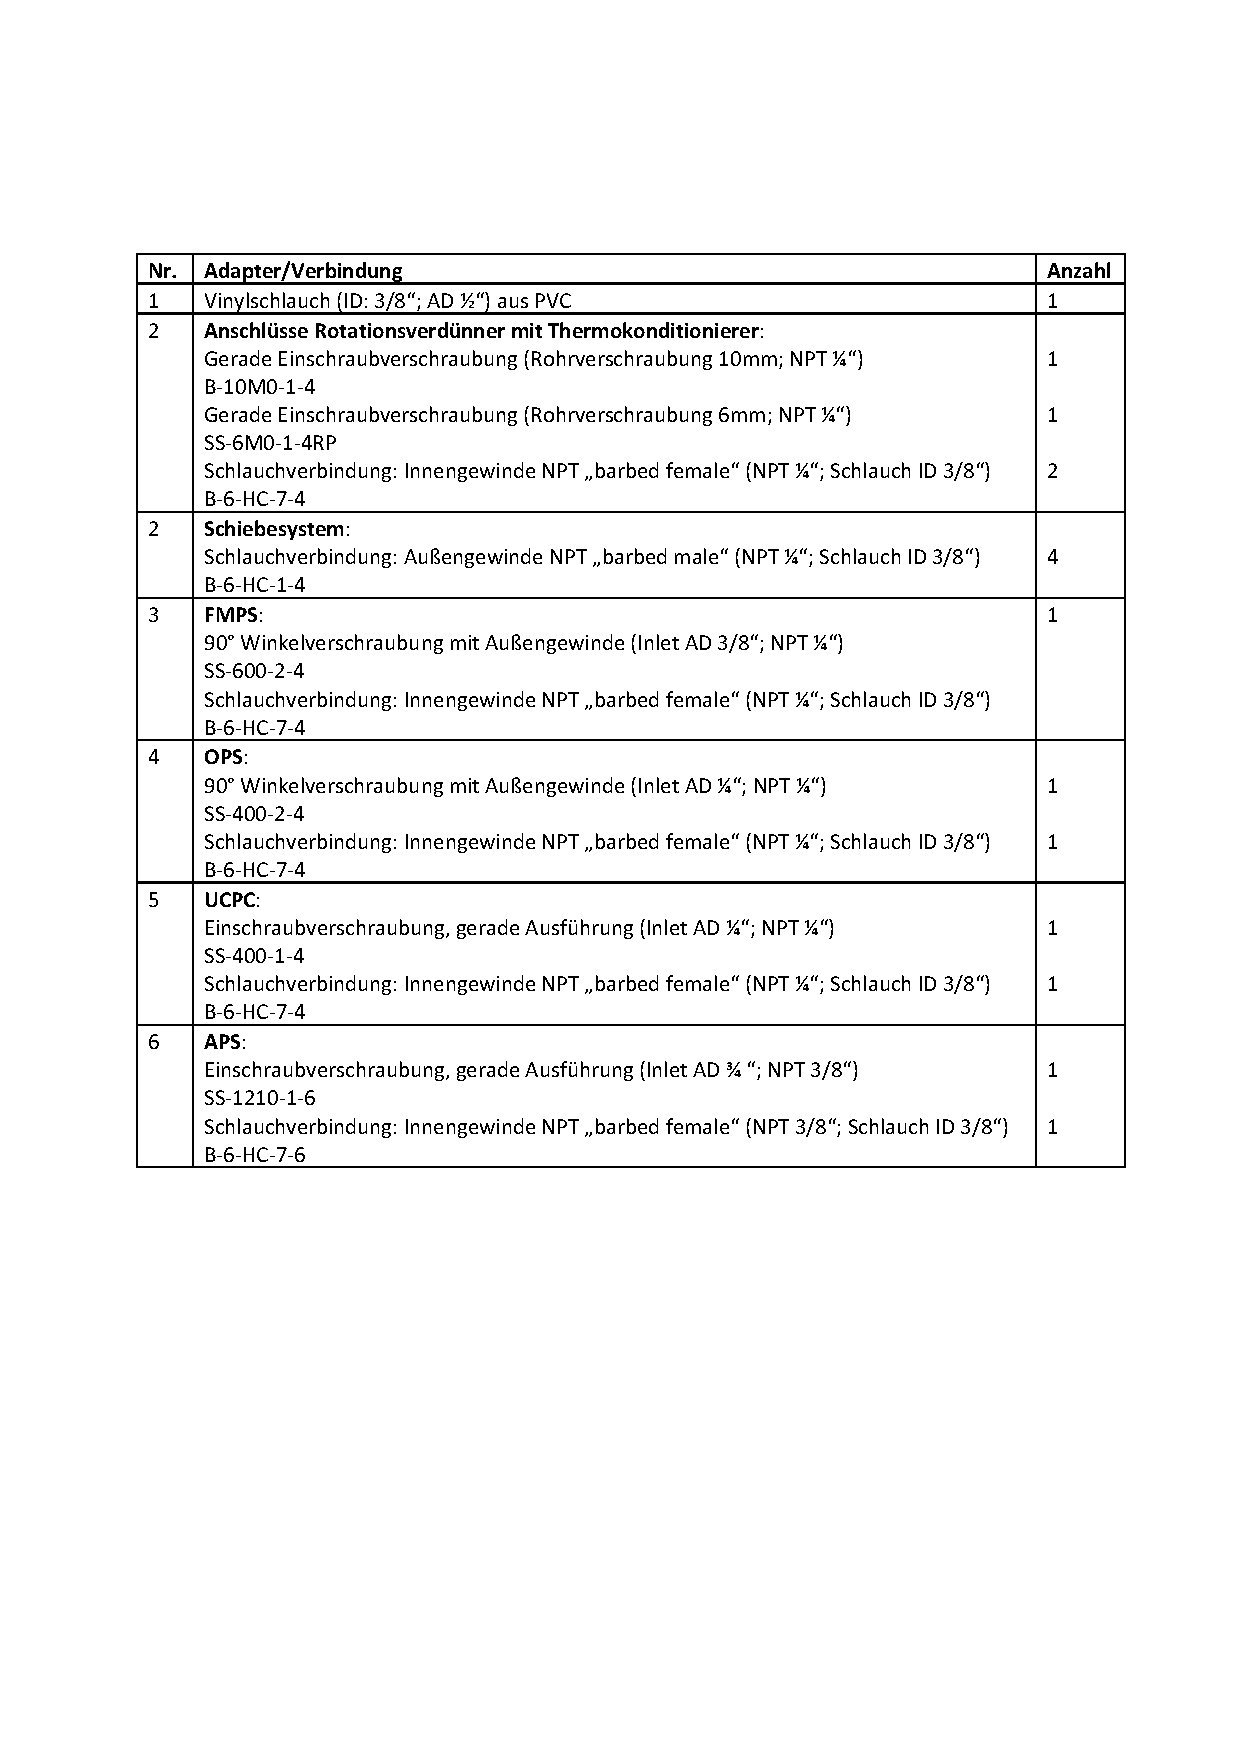
\includegraphics[width=.9\linewidth]{gfx/construction/material.pdf}} \quad
        \caption[Verbindungen und Adapter]
        {Verbindungen und Adapter}
        \label{fig:material}
\end{figure}
Der Rotationsverd\"{u}nner ben\"{o}tigt zwei Einschraubverschraubungen mit einem \(\textit{NPT} \frac{1}{4} inch\) Au{\ss}engewinde. Zum Verbinden der Schl\"{a}uche dienen somit die Schlauchverbindungen mit einem Innengewinde \(\textit{NPT} \frac{1}{4} inch\) und einem Zapfen passend f\"{u}r Schl\"{a}uche mit einem Innendurchmesser von \(\frac{3}{8} inch\). Auf Grundlage dieser Anschl\"{u}sse haben die weiteren Anschl\"{u}sse der Verbindungsplatte und der Drehscheibe die gleichen Innengewinde. Somit werden jeweils zwei Schlauchverbindungen an der Verbindungsplatte und an der Drehscheibe ben\"{o}tigt.
\\\\
Die Eing\"{a}nge der Messger\"{a}te sind verschieden positioniert und haben unterschiedliche Anschlussdurchmesser. Daher sind f\"{u}r jedes Messger\"{a}t Adapter notwendig, die an die Versuchseinrichtung angeschlossen werden k\"{o}nnen. Um Verschlei{\ss}erscheinungen, die durch Knicken des Schlauches entstehen, werden f\"{u}r den \textit{FMPS} und \textit{OPS} \(90^\circ\) Winkelverschraubungen genutzt. F\"{u}r den \textit{APS} und \textit{UCPC} werden Einschraubverbindungen in gerader Ausf\"{u}hrung verwendet. Die Verbindung zum Schlauch wird durch eine Schlauchverbindung mit Innengewinde hergestellt. Diese wird auf den Adapter f\"{u}r das jeweilige Messger\"{a}t geschraubt.
\\\\
Als Verbindung zu den Elementen der Versuchseinrichtung werden Vinylschl\"{a}uche verwendet. Der Vinylschlauch ist in Rollen erh\"{a}ltlich und kann zu den gew\"{u}nschten L\"{a}ngen zerschnitten werden. Neue Schl\"{a}uche gelten als technisch glatt\citep{grote} und eignen sich daher f\"{u}r die Versuchseinrichtung. Zur Verteilung der Bewegungen und Biegungen, die unter dem Mindesbiegeradius des Schlauches liegen und aufgrund des Messger\"{a}tebewegtoleranz ist der Schlauch mit ausreichender L\"{a}nge zu w\"{a}hlen. Damit werden fr\"{u}he Verschlei{\ss}erscheinungen vermieden. Unter den Bedingungen der Schlauchverbindungen und der Schlauchf\"{u}hrung ergeben sich folgende Schlauchl\"{a}ngen:
\begin{enumerate}
	\item Kerze zum Verd\"{u}nner: \(480mm\)
	\item Verd\"{u}nntes Aerosol zur Verbindungsplatte: \(160mm\)
	\item HEPA-Filter zur Verbindungsplatte: \(280mm\)
	\item Drehscheibe zum Verdichter: \(240mm\)
	\item Drehscheibe zum Messger\"{a}t: \(240mm\)
\end{enumerate}
Je nach Variation des Aufbaus k\"{o}nnen die Schlauchl\"{a}ngen variieren. Da Vinylschl\"{a}uche einfach in ihrer Beschaffenheit und kosteng\"{u}nstig sind, k\"{o}nnen die Schl\"{a}uche nach Belieben verl\"{a}ngert oder verk\"{u}rzt werden.
\\\\
Die Entscheidung zugunsten eines rotatorischen Schiebers fiel aus mehreren Gr\"{u}nden. Rotatorische Schritt- oder Servomotoren werden gro{\ss}fl\"{a}chig angeboten und sind dazu sehr preisg\"{u}nstig. Die Auslegung des Rotors und des Stators sind konstruktiv einfacher zu realisieren, da diese aus einfachen Grundgeometrien gefertigt werden k\"{o}nnen, w\"{a}hrend der translatorische Schieber die Konstruktion einer komplexen Schiene und einer \"{U}bertragungswelle ben\"{o}tigt. Die Ansteuerung eines rotatorischen Aktuators erweist sich au{\ss}erdem als weniger aufw\"{a}ndig und g\"{u}nstiger, da die Rotationsbewegungen aus dem Motor direkt \"{u}ber Software auslesbar ist, w\"{a}hrend bei einem translatorischen System komplizierte Umrechnungen notwendig sind. Das Ansaugen des Aerosols durch einen Verdichter, sowie der horizontale Verlauf der Str\"{o}me durch den Rotor, tragen zu einem str\"{o}mungsbeg\"{u}nstigendem Schaltvorgang bei.
\\\\
Als bewegliche Komponente ist der Rotor f\"{u}r den Wechsel zwischen Luftstrom und konditioniertem Aerosolstrom zust\"{a}ndig. Die daf\"{u}r notwendige mechanische Energie wird durch einen Schrittmotor zur Verf\"{u}gung gestellt. Der Rotor besteht aus einer 3-D gedruckten, runden Scheibe aus Polyamid mit folgenden Ma{\ss}en:
\begin{enumerate}
	\item Durchmesser: \(120 mm \pm 5 mm\)
	\item Dicke: \(11,5 mm \pm 1 mm\)
\end{enumerate}
Auf der dem Stator abgewandten Seite sind auf einem zum Rotor konzentrischen Kreis mit dem Radius \(4 mm\) zwei durchg\"{a}ngige konische Bohrungen. Die Bohrungen verj\"{u}ngen sich zur R\"{u}ckseite hin und besitzen jeweils ein \(\frac{1}{4} inch\) Innengewinde. Der Winkel zwischen den beiden Bohrungen betr\"{a}gt \(43,2^\circ\). Des Weiteren besitzt die Scheibe eine durchg\"{a}ngige Bohrung mit einem Radius von \(2,5 mm \pm 0,01 mm\) in ihrem Zentrum. Auf der R\"{u}ckseite des Rotors befindet sich eine Matte aus technischem Filz in Form eines symmetrischen Kreissegmentes mit folgenden Ma{\ss}en:
\newpage
\begin{enumerate}
	\item Dicke: \(4 mm \pm 1mm\)
	\item Radius: \(60 mm \pm 2 mm\)
	\item H\"{o}he in der Mitte: \(50 mm \pm 2 mm\)
\end{enumerate}
Die Matte ist auf der R\"{u}ckseite des Rotors mit diesem verklebt. Dabei liegt ihre Symmetrieachse mittig zwischen den beiden Bohrungen und die abgerundete Seite ist konzentrisch zur Scheibe angeordnet. An den Stellen der Bohrung ist die Matte mit kreisf\"{o}rmigen Ausschnitten versehen, welche konzentrisch zu den Bohrungen liegen. Der Durchmesser der Ausschnitte ist je \(1 mm\) gr\"{o}{\ss}er als der der Bohrungen. Der Rotor ist auf die Antriebswelle des Aktuators geschoben, sodass die Filzmatte durch den Stator leicht eingedr\"{u}ckt ist.
\\\\
Der Stator dient der Aufnahme der Kr\"{a}fte und Momente, welche durch den Schaltvorgang entstehen. Bei der Auswahl der Geometrie spielt auch die Funktion des Stators als Schlauchhalter eine Rolle. Au{\ss}erdem ist ein Material gew\"{a}hlt worden, mit welchem eine Dichtung trotz Relativbewegung realisierbar ist. Der Stator besteht aus einer Platte geh\"{a}rtetem Stahl, mit folgenden Ma{\ss}en:
\begin{enumerate}
	\item Tiefe: \(11,5 mm \pm 1 mm\)
	\item H\"{o}he: \(140 mm \pm 5mm\)
	\item Breite: \(110 mm \pm 5 mm\)
\end{enumerate}
Auf der dem Rotor abgewandten Seite befindet sich in H\"{o}he von \(70 mm\) und in der halben Breite \(55 mm\) eine durchgehende Bohrung mit dem Radius von \(3,5 mm \pm 0,25 mm\). In diese Bohrung ist die Antriebswelle des Motors eingef\"{u}hrt, sodass sie circa \(1 mm\) Spiel hat. Der Motor ist in dieser Position durch vier \textit{M3 x 12 Senkkopfschrauben} am Stator fixiert. Au{\ss}erdem ist zur Stabilisierung des Motors ein \( 40mm * 40 mm * 40 mm\) Edelstahlwinkel so am Startor angebracht, dass die Unterseite des Motors auf dem Winkel aufliegt. Der Stator selbst ist mit Hilfe von zwei \(40mm * 40mm * 30mm\) Edelstahlwinkeln an einer Grundplatte montiert. Auf einem zum Umfang der Antriebswelle konzentrischen Kreis mit \(40mm\) Radius befinden sich zwei um \(\pm 21,6^\circ\) von der 12-Uhr-Position versetzten, konisch zulaufende Durchgangsbohrungen, welche sich zum Rotor hin verj\"{u}ngen. In diesen Bohrungen sind jeweils \(\frac{1}{4} inch\) \textit{NPT} Innengewinde geschnitten. zus\"{a}tzlich befindet sich auf der R\"{u}ckseite eine, um \(64,8^\circ\) von der 12-Uhr-Position aus, gegen den Uhrzeigersinn versetzte, durchgehende Bohrung, mit einem Radius von \(5mm\). Die Bohrungen sind auf der Vorderseite mit je einer \(45^\circ\)-Fase versehen, welche der Abrasion der Filzmatte durch scharfe Bohrkanten vorbeugt.
\\\\
Als Aktuator f\"{u}r die Schaltvorrichtung wird der Schrittmotor \textit{QSH4218-41-10-035} der Firma \textit{Trinamic} benutzt. Der Motor hat ein Halte-Drehmoment von \(0,35 NM\) und l\"{a}sst sich \"{u}ber eine Schnittstelle mit einem \textit{Trinamic Board} \"{u}ber passende Software ansteuern. Die Antriebswelle hat eine L\"{a}nge von \(20 mm\) und einen Durchmesser von \(5 mm\). Der Motor hat sich aufgrund des g\"{u}nstigen Preises und der einfachen Ansteuerung durchgesetzt. Die Firma baut eigens f\"{u}r den Motor ein passendes Board zur digitalen Ansteuerung. Dabei wird der Motor mit einem \textit{RS-485 Kabel} mit dem Board verbunden, welches direkt per \textit{USB} mit einem Computer verbunden werden kann. Das Board l\"{a}sst sich frei programmieren und so kann man verschiedene Schaltvorg\"{a}nge implementieren.
\\\\
Abschlie{\ss}end wurde noch eine schematische Darstellung gefertigt (Abbildung \ref{fig:scheme}), welche zeigt wie die einzelnen Elemente des Aufbaus zusammen geh\"{o}ren.
\begin{figure}[H]
        \myfloatalign
        {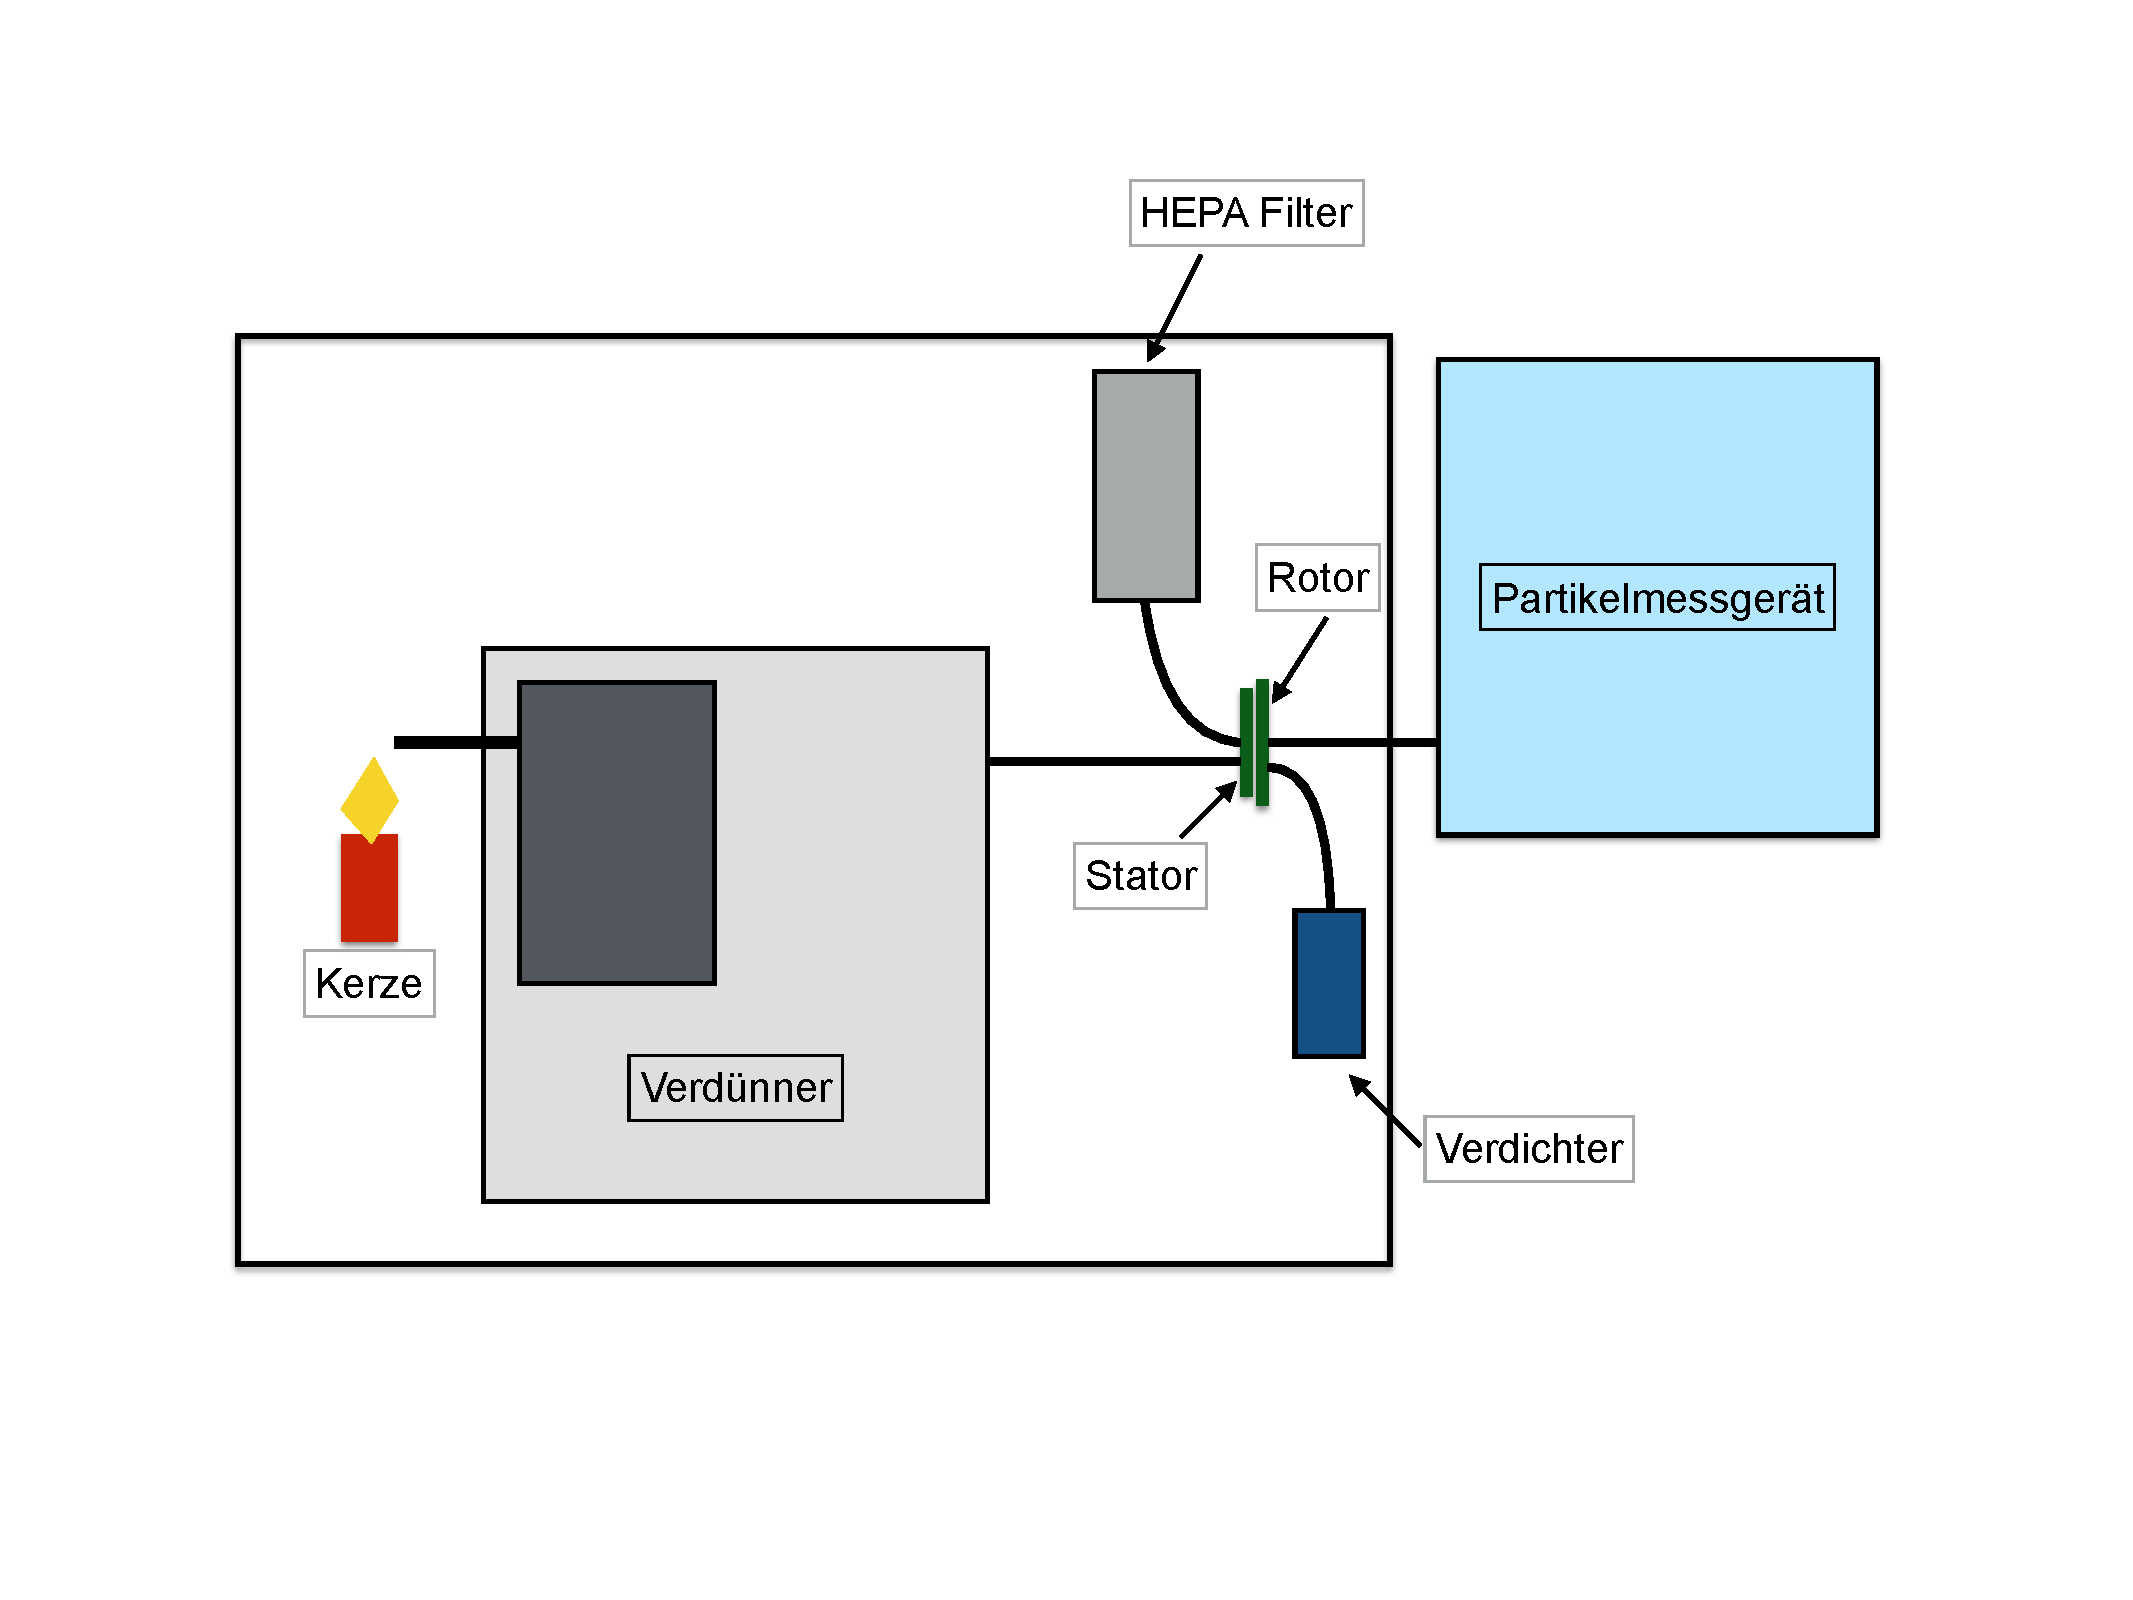
\includegraphics[width=.9\linewidth]{gfx/conclusion/aufbau.pdf}} \quad
        \caption[Schematische Darstellung des Versuchaufbaus]
        {Schematische Darstellung des Versuchaufbaus}
        \label{fig:scheme}
\end{figure}

\subsection{Durchf\"{u}hrung des Versuchs}
F\"{u}r eine Analyse des dynamischen Verhaltens der Messger\"{a}te sind vor allem deren Totzeiten und die Genauigkeit der ersten Messwerte im Vergleich zu den folgenden Messwerten interessant. Um eine Aussauge \"{u}ber die Totzeit des Messger\"{a}tes treffe zu k\"{o}nnen, muss aus der gesamten Totzeit des Systems, die Totzeit des Versuchsaufbaus abgezogen werden. Diese wird beschrieben durch die Dauer zwischen Generieren des Schaltsignals und dem Ankommen der Partikelfront am Messger\"{a}teeinlass. Ein Anteil dieser Zeitspanne ist die Schaltzeit des Rotors welche bei \(t_s = 0,4 s\) liegt. Der restliche Anteil ist die Zeit, die der Volumenstrom ben\"{o}tigt um von der Schaltvorrichtung bis zum Messger\"{a}teeinlass zu gelangen und errechnet sich aus:
\begin{align*}
t_w = \frac{s * \pi * r^2}{V'}
\end{align*} 
mit \(s = \textit{Wegstrecke zwischen Schaltvorrichtung und Messger\"{a}teeinlass} = 250 mm\), \(r = \textit{Schlauchradius} = 4,7625 mm\) und \(V' = \textit{Volumenstrom des Messger\"{a}tes}\).\\
Damit diese Beziehung gilt muss das Verhalten der Str\"{o}mung im Schlauch zum Messger\"{a}t laminar sein. Um zu zeigen, dass dies erf\"{u}llt ist, wird unter Vernachl\"{a}ssigung der Querschnitts\"{u}berg\"{a}nge am Messger\"{a}teeinlass und am Rotorauslass, im Folgenden die Reynoldszahl f\"{u}r diesen Weg berechnet. Dabei ist zu erw\"{a}hnen, dass nur die Durchf\"{u}hrung am \textit{FMPS} betrachtet wird, da dieser den h\"{o}chsten Volumendurchsatz besitzt und die anderen Parameter unabh\"{a}ngig vom Messger\"{a}t sind.
\begin{align*}
Re = \frac{2V'}{r * \pi * \nu_\textit{Luft}} = 137 < 2300
\end{align*}
wobei \(V' = 1,67*10^{-5}\frac{m^3}{s}\), \(r = 4,7625 * 10^{-3}m\) und \(\nu_\textit{Luft}(30^\circ C) = 163 * 10^{-7} \frac{m^2}{s}\).
Daraus folgt, dass sich der Strom bei isolierter Betrachtung dieses Weges laminar verh\"{a}lt. Weiterhin ergeben sich nun die Totzeiten unseres Versuchsaufbaus abh\"{a}ngig von den verschiedenen Messger\"{a}ten durch\\
\(t_\textit{Versuch, Messger\"{a}t} = t_w + t_s\):
\begin{itemize}
	\item \(t_\textit{Versuch, FMPS} = 0,507s\)
	\item \(t_\textit{Versuch, APS} = 0,614s\)
	\item \(t_\textit{Versuch, OPS} = 1,47s\)
	\item \(t_\textit{Versuch, UCPC} = 1,11s\)
\end{itemize}
Da bei der Kerze als Aerosolquelle eine relativ hohe Streuung der Partikelanzahlkonzentrationswerte zu erwarten ist, muss der Pr\"{u}fvorgang mehrere Pr\"{u}fdurchg\"{a}nge enthalten. Die hohe Filterwirkung des \textit{HEPA-Filters} garantiert hierbei trotzdem, dass die minimale Partikelanzahlkonzentrationsdifferenz eingehalten wird.\\
Der Pr\"{u}faufbau sieht folgenderma{\ss}en aus:
\begin{enumerate}
	\item Alle Schl\"{a}uche werden auf die f\"{u}r sie vorgesehene Steckpl\"{a}tze gesteckt. 
	\item Das Messger\"{a}t wird mit dem Versuchsaufbau verbunden.
	\item Die Kerzen werden angez\"{u}ndet.
	\item Der Motor wird angeschaltet und In \textit{Stellung 0} gebracht.
	\item Das Messger\"{a}t und die Pumpe werden angeschaltet.
\end{enumerate}
Nachdem sich die Pumpe und das Messger\"{a}t eingelaufen haben und die erw\"{u}nschten Volumenstr\"{o}me erreicht sind kann die eigentliche Pr\"{u}fdurchf\"{u}hrung beginnen. Je nach Messger\"{a}t wird zuerst der Zeitpunkt des Eintreffens der Partikelfront auf den Messger\"{a}teeinlass nach der Schaltung bestimmt. Dies passiert in Abh\"{a}ngigkeit der vorher berechneten Totzeit \(t_\textit{Versuch, Messger\"{a}t}\). Der Rotor wird jetzt in \textit{Stellung 1} gebracht und das gemessene Partikelsprungsignal wird aufgezeichnet. Der Partikelmesswert nach dem Sprung wird abgespeichert und der Rotor wird wieder in \textit{Stellung 0} geschaltet. Ist der Nullwert wieder erreicht kann die n\"{a}chste Messung durchgef\"{u}hrt werden.\\
Um das Ergebnis der Versuchseinrichtung als valide annehmen zu k\"{o}nnen muss eine statistische Messreihe erstellt werden. Daf\"{u}r werden nun so viele Versuche durchgef\"{u}hrt, bis das arithmetische Mittel der Messreihe sich nicht mehr ausschlaggebend \"{a}ndert. Eine Messreihe wird von uns als valide angenommen wenn die Mittelwert\"{a}nderung unter \(0,001\) ist, der Wert also eine Genauigkeit von \(99,9\%\) angenommen hat.

\subsection{Kosten}
F\"{u}r die Kosten des Versuchsaufbaus wurden die Kosten von jedem Bauteil ermittelt und aufsummiert. Dabei ist zu beachten, dass nicht alle Preise fest zu sehen sind, da sie immer nur auf Nachfrage bei den Herstellern herausgegeben werden und sich eventuell \"{a}ndern k\"{o}nnen. Die Kosten f\"{u}r die 3-D gedruckten Teile wurden aus Erfahrungswerten und dem Preis f\"{u}r 3-D Druck Material ermittelt.\\
Die Gesamtkosten sind in folgender Tabelle \ref{fig:kosten} einzusehen:
\begin{figure}[H]
        \myfloatalign
        {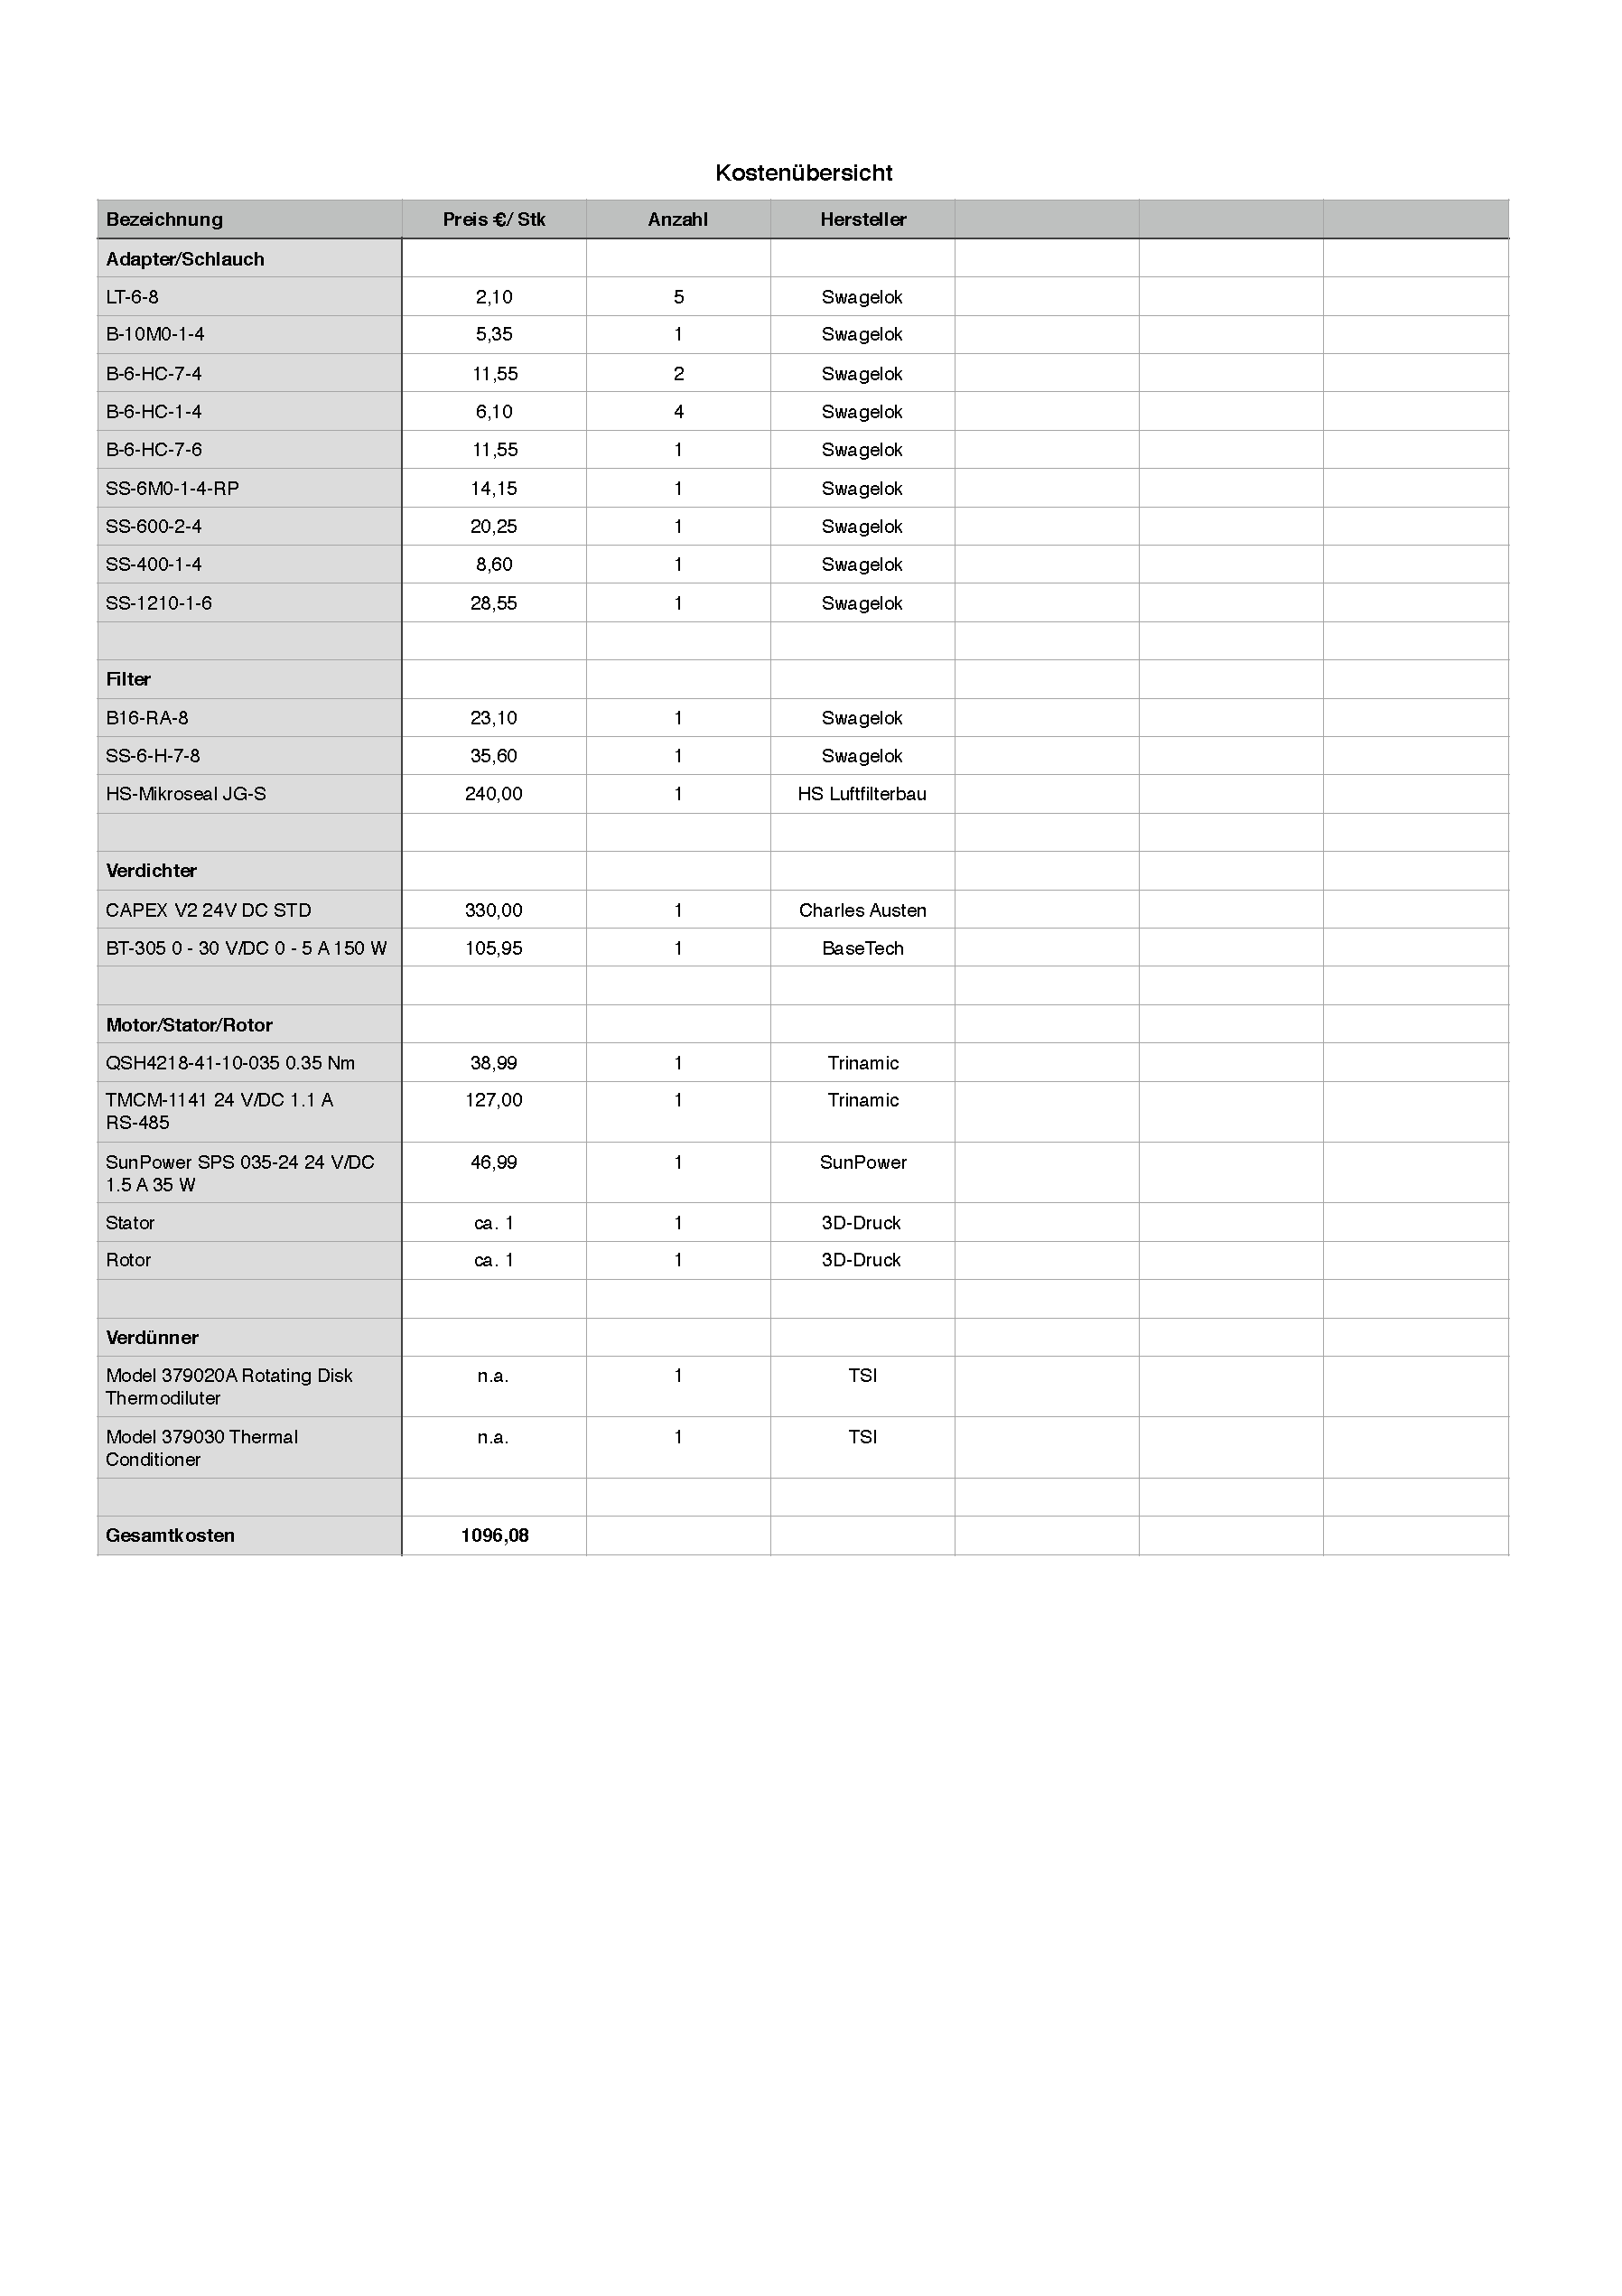
\includegraphics[width=.9\linewidth]{gfx/construction/kosten.pdf}} \quad
        \caption[Kosten aller Teile]
        {Kosten aller Teile}
        \label{fig:kosten}
\end{figure}

\subsection{Evaluation}
Die Genauigkeit und Korrektheit des Versuchs h\"{a}ngt ma{\ss}geblich von zwei Faktoren ab. Einmal von den Druckverh\"{a}ltnissen in den Schl\"{a}uchen und Verbindungen und andererseits von der Schaltzeit des Rotors.\\
Die folgende Druckberechnung verdeutlicht die Druckdifferenz, die aufgrund der Schlauch und Schlauchverbindungsreibungen  zwischen dem
Rotationsverd\"{u}nner und dem Messger\"{a}teingang anf\"{a}llt. Die Schlauchverbindungen bestehen aus Messing und die Schl\"{a}uche aus Polyvinylchlorid (weiches PVC). Da das Aerosol des Kerzenrauchs im Rotationsverd\"{u}nner verd\"{u}nnt wird, ist f\"{u}r den Druckgradienten am Messger\"{a}teinlass der Weg vom Verd\"{u}nner aus relevant. Dieser betr\"{a}gt ungef\"{a}hr 
\begin{align*}
l_{gesamt} = l_{Messing} + l_{PVC} = 170mm + 320mm = 530mm
\end{align*}
Der Druckgradient berechnet sich zu
\begin{align*}
\Delta p_\textit{Messger\"{a}t} = \zeta_\textit{Messing} \frac{l_\textit{Messing}}{d_\textit{Messing}}\frac{\rho * u^{2}_\textit{Messger\"{a}t, Messing}}{2} + \zeta_\textit{PVC} \frac{l_\textit{PVC}}{d_\textit{PVC}} \frac{\rho * u^{2}_\textit{Messger\"{a}t, PVC}}{2}
\end{align*} 
\begin{center}
\begin{tabular}{c | c}
$\zeta_{i}$ & Widerstandsbeiwert\\
\hline
$d_{i}$ & Innendurchmesser der Verbindung\\
\hline
$\rho$ & Dichte des Volumenstroms\\
\hline
$u_{j,i}$ & Geschwindigkeit des Aerosolstroms,\\
& die sich aus dem Volumenstrom ergibt,\\
& welchen die Messger\"{a}te erzeugen
\end{tabular}
\end{center}
F\"{u}r laminare Str\"{o}mungen l\"{a}sst sich der Rohrreibungskoeffizient nach dem Gesetz von Hagen-Poiseuille bestimmen:
\[\lambda_{i} = \frac{64}{Re_{i}}=\zeta_{i}\]
\[\zeta_{Messing_\textit{max}} = 0,0015\]
\[\zeta_{PVC_\textit{max}} = 0,0015\]
Es kann die Dichte des Tr\"{a}gergases angenommen werden. Diese betr\"{a}gt bei $25^{\circ}C$ \[\rho = 1,18 \frac{kg}{m^{3}}\]\\
Des Weiteren betragen die Durchmesser
\[d_{Messing} = 4,8 mm\]
\[d_{PVC} = 9,5 mm\]
Im Folgenden wird nur die Druckdifferenz, die bei Nutzung des  FMPS entsteht, berechnet. Da dieser den h\"{o}chsten Volumenstrom aller verwendeten Messger\"{a}te erzeugt, ist folglich die Geschwindigkeit des Aerosolstroms hier am gr\"{o}{\ss}ten. Relevant ist diese Druckdifferenz, da die Druckgradienten bei der Nutzung der anderen Messger\"{a}te geringer ausfallen.
\\\\
Mit den Geschwindigkeiten des Aerosolstroms \[u_{FMPS, Messing} = 9,21 \frac{m}{s}\] \[u_{FMPS, PVC} = 2,35 \frac{m}{s}\] ergibt sich der Druckunterschied f\"{u}r den FMPS zu \[\Delta p_{FMPS} = 2,8 Pa\]
\\\\
Aufgrund der Wahl von technisch glatten Rohren und der kurzen Versuchsstrecke sind die entstehenden Druckgradienten f\"{u}r die Messger\"{a}te vernachl\"{a}ssigbar und k\"{o}nnen ohne weitere Probleme ausgeglichen werden.
\\\\
Der zweite Faktor ist die Schaltzeit die unter anderem vom Motor abh\"{a}ngt. Dazu wurde die Schaltzeit mit dem verwendeten Motor mit allen wichtigen Komponenten berechnet. F\"{u}r die folgende Rechnung wurde zur Vereinfachung die Reibung der Filzdichtung ignoriert.
Momentengleichung um Rotorachse:
\[M_\textit{Rotor}: \Theta * \phi'' = M_M\]
\[\Rightarrow M_M = \frac{2*\phi*\Theta}{t^2}\]
\[\Rightarrow t = \sqrt{\frac{2*\phi*\Theta}{M_M}}\]
\[M_M = 0,35Nm\]
\[\phi = 43,2^\circ = 0,754 \textit{rad}\]
Das Fl\"{a}chentr\"{a}gheitsmoment ergibt sich zu:
\[\Theta = \Theta_\textit{Scheibe} + \Theta_{Adapter} + 2m_\textit{Adapter} * d^2\]
\[d = 4 * 10^{-2}m\]
\[n_\textit{Adapter} = 0,018kg\]
\[\Theta_\textit{Scheibe} = \frac{1}{2}*m_\textit{Scheibe} * r^2 = \frac{1}{2} * 1140\frac{kg}{m^3}*\pi *(6*10^{-2}m)^2 * 1,15 * 10^{-2}m = 0,0236kgm^2\]
\[\Theta_\textit{Adapter} = \frac{m*(r_1^2+r_2^2)}{2} = \frac{0,018kg * ((7,6*10^{-2}m)^2+(16,6*10^{-2}m)^2)}{2} = 3*10^{-4}kgm^2\]
\[\Rightarrow \Theta = 0,02426kgm^2\]
\\\\
\[\Rightarrow t = \sqrt{\frac{2*0,754\textit{rad}*0,02426 kgm^2}{0,35Nm}} = 0,3233s\]
\\\\
Mit gew\"{a}hltem Motor l\"{a}sst sich also eine Schaltzeit von \(0,3233s\) erreichen, was die angestrebte Schaltzeit von \(0,4s\) unterschreitet und somit f\"{u}r den Versuchsaufbau ausreichend ist.\\

